\chapter{Resultados y discusión}
\label{cap:resultados}

Este capítulo presenta los resultados registrados en el CSV maestro del experimento. El análisis se realizó sobre el experimento principal, conservando la correspondencia entre cada imagen, la réplica, la profundidad, la repetición técnica y el método de conversión métrica. Las cifras se informan como una comparación dentro del montaje utilizado y contra las referencias físicas de las réplicas; no se interpretan como una validación del sistema en otras condiciones.

\section{Composición del conjunto y control de calidad}
\label{sec:conjunto}

El archivo contiene 288 registros: 72 imágenes, seis réplicas de PLA, cuatro posiciones nominales respecto del vidrio (5, 11, 17 y 23~cm), tres capturas técnicas por condición y cuatro métodos (A, \Aprime, B y C). Por cada combinación de réplica y profundidad se dispone, en general, de tres capturas. Las capturas repetidas se trataron como repeticiones técnicas y no como réplicas independientes.

Se obtuvieron valores numéricos para 284 registros. Los cuatro registros sin medición corresponden a A y \Aprime{} en dos imágenes en las que no se detectó el marcador ArUco: \texttt{R2-REP2-170.jpg} y \texttt{R3-REP2-50.jpg}. El motivo se conservó en el CSV y esos registros se excluyeron de los cálculos de error. Los métodos B y C produjeron valores para las 72 imágenes. La aplicación conserva para ambos un estado interno \texttt{PENDING\_VALIDATION}, que solo cambia cuando se registra una barra patrón sumergida; esa comprobación instrumental complementaria no se realizó (Sección~\ref{sec:metodos}). La validación métrica de B y C en este trabajo es la comparación directa con las longitudes y profundidades de calibre de las seis réplicas en las cuatro posiciones, que se presenta en las Secciones~\ref{sec:agregados} y~\ref{sec:profundidad}. La Tabla~\ref{tab:registros} resume el tratamiento de los registros.

\begin{table}[htbp]
\centering\small
\caption{Registros del CSV y su tratamiento en el análisis.}
\label{tab:registros}
\begin{tabular}{@{}lccp{7.5cm}@{}}
\toprule
Método & Registros & Con valor & Tratamiento \\
\midrule
A & 72 & 70 & Se excluyeron dos registros por falta de detección del ArUco. \\
\Aprime & 72 & 70 & Se excluyeron dos registros por falta de detección del ArUco. \\
B & 72 & 72 & Valor numérico en las 72 imágenes; evaluado contra la referencia de calibre. \\
C & 72 & 72 & Valor numérico en las 72 imágenes; evaluado contra la referencia de calibre. \\
\bottomrule
\end{tabular}
\end{table}

En las dos combinaciones afectadas por la ausencia de ArUco, A y \Aprime{} se promediaron con las dos capturas disponibles, mientras que B y C usaron las tres; el pareamiento no es por ello idéntico en esas dos combinaciones. Al repetir el cálculo de las Tablas~\ref{tab:agregados} y~\ref{tab:posiciones-mae} solo con las 70 imágenes comunes a los cuatro métodos, ningún valor cambió en más de 0,01~mm o 0,01 puntos porcentuales, y los conteos de la comparación pareada de la Sección~\ref{sec:agregados} se mantuvieron; los resultados no dependen de esas dos capturas.

\section{Calibraciones}
\label{sec:calibraciones}

Las dos calibraciones de cámara se realizaron el 12 de octubre de 2026 con el damero de $4 \times 4$ esquinas interiores y cuadros de 20~mm, a la resolución de captura de $4096 \times 3072$ píxeles. La Tabla~\ref{tab:calibraciones} resume sus indicadores de calidad; los perfiles completos se reproducen en el Anexo~\ref{anx:calibraciones}.

\begin{table}[htbp]
\centering\footnotesize
\caption{Calibraciones de cámara utilizadas por las rutas B y C.}
\label{tab:calibraciones}
\begin{tabular}{@{}p{4.2cm}p{4.4cm}p{4.4cm}@{}}
\toprule
Campo & Perfil B (bajo agua) & Perfil C (en aire) \\
\midrule
Identificador & \texttt{B-effective} & \texttt{C-air} \\
Rutina & \texttt{calibrateCamera} (OpenCV 5.0.0) & \texttt{calibrateCamera} (OpenCV 5.0.0) \\
RMS de reproyección & 0,4354~px & 0,3745~px \\
Vistas recibidas / aceptadas & 35 / 35 & 36 / 36 \\
Vistas rechazadas & 0 & 0 \\
Focal efectiva $f_x$ & 4502,3~px & 3313,7~px \\
Punto principal $(c_x, c_y)$ & (2027,3; 1549,0)~px & (2028,2; 1530,6)~px \\
\bottomrule
\end{tabular}
\end{table}

Ambos valores de RMS están por debajo de 0,5~px, umbral habitual para una calibración aceptable, y ninguna vista fue rechazada. La razón entre las focales efectivas, $f_{x,\mathrm{agua}}/f_{x,\mathrm{aire}} = 4502{,}3/3313{,}7 = 1{,}36$, es consistente con el índice de refracción del agua ($\mu_w = 1{,}333$): la calibración de B absorbe la refracción en una focal efectiva mayor. Para incidencia cercana a la normal, un puerto plano equivale en primer orden a una cámara pinhole con la focal multiplicada por $\mu_w$ y el centro de proyección desplazado, de modo que el modelo efectivo puede reproducir la escala a distintas profundidades si el plano de medición se ubica correctamente; los efectos no centrales que lo hacen depender de la distancia crecen con el ángulo de incidencia \parencite{Rofallski2022}.

\subsection{Sensibilidad de C a los parámetros del montaje}
\label{sec:sensibilidad}

\begin{table}[htbp]
\centering\footnotesize
\caption{Sensibilidad de la longitud total estimada por C a los parámetros medidos a mano: cambio medio con signo sobre las 72 capturas respecto de la configuración base ($d = 230$~mm, $\mu_w = 1{,}333$).}
\label{tab:sensibilidad}
\begin{tabular}{@{}p{4cm}p{2.6cm}p{2.8cm}p{2.8cm}@{}}
\toprule
Parámetro & Variación & Cambio medio de LT (mm) & Cambio medio de LT (\%) \\
\midrule
Distancia cámara--vidrio $d$ & $-20$~\% (184~mm) & $-20{,}57$ & $-14{,}01$ \\
Distancia cámara--vidrio $d$ & $+20$~\% (276~mm) & $+20{,}57$ & $+14{,}01$ \\
Índice del agua $\mu_w$ & $-0{,}01$ (1,323) & $+0{,}34$ & $+0{,}23$ \\
Índice del agua $\mu_w$ & $+0{,}01$ (1,343) & $-0{,}33$ & $-0{,}23$ \\
\bottomrule
\end{tabular}
\end{table}

C se recalculó sobre las 72 capturas con cada variante, conservando la distancia $z$ de la réplica a la cara interna del vidrio; al cambiar $d$ se desplazaron tanto la interfaz como el plano de medición. Un error de $\pm 20$~\% en $d$ ($\pm 46$~mm) cambió la LT en 20,57~mm (14,01~\%) en promedio, en concordancia con la aproximación de primer orden de la ecuación~\eqref{eq:Dz}, según la cual una variación $\Delta d$ cambia la longitud estimada en una fracción $\Delta d / D(z)$, con $D(z)$ entre 270 y 405~mm en las posiciones estudiadas. Esto equivale a cerca de 0,3~\% de LT por milímetro de error en $d$: un error de 5~mm ya supera el MAPE de C (0,88~\%). La distancia cámara--vidrio es, por tanto, el parámetro del montaje que más condiciona la exactitud de C y debe medirse con cuidado. En cambio, una variación de $\pm 0{,}01$ en $\mu_w$ cambió la LT en 0,34~mm (0,23~\%) en promedio y en no más de 0,70~mm en una captura individual, por debajo del MAE de C, de modo que el uso de un índice tabulado no limitó la exactitud.

\section{Resultados agregados por método}
\label{sec:agregados}

Las métricas se calcularon según la Sección~\ref{sec:evaluacion} después de promediar las tres capturas de cada combinación réplica--profundidad, de modo que la comparación principal quedó formada por 24 combinaciones por método. La Tabla~\ref{tab:agregados} resume las diferencias entre las estimaciones promediadas y sus referencias físicas, y la Figura~\ref{fig:4-1} las presenta gráficamente. A presenta sesgo negativo en ambas medidas, mientras que \Aprime{} y C tienden a sobreestimar; B tiene un sesgo prácticamente nulo en LT ($+0{,}05$~mm) y levemente negativo en PC ($-0{,}32$~mm). B y C obtienen los menores errores, con valores cercanos entre sí; \Aprime{} queda en tercer lugar y A es el método más afectado.

\begin{table}[htbp]
\centering\footnotesize
\caption{Errores medios por método después de resumir las repeticiones técnicas.}
\label{tab:agregados}
\begin{tabular}{@{}lccccccccc@{}}
\toprule
 & & \multicolumn{6}{c}{Promedio por combinación} & \multicolumn{2}{c}{Por captura} \\
\cmidrule(lr){3-8}\cmidrule(l){9-10}
Método & $n$ & Sesgo LT & MAE LT & MAPE LT & Sesgo PC & MAE PC & MAPE PC & MAE LT & MAE PC \\
 & & (mm) & (mm) & (\%) & (mm) & (mm) & (\%) & (mm) & (mm) \\
\midrule
A       & 24 & $-37{,}43$ & 37,43 & 25,68 & $-9{,}07$ & 9,07 & 25,25 & 37,75 & 9,16 \\
\Aprime & 24 & $+3{,}29$  & 3,29  & 2,28  & $+0{,}95$ & 1,03 & 2,78 & 3,33 & 1,03 \\
B       & 24 & $+0{,}05$  & 1,08  & 0,73  & $-0{,}32$ & 0,38 & 1,26 & 1,35 & 0,54 \\
C       & 24 & $+1{,}07$  & 1,22  & 0,88  & $+0{,}29$ & 0,56 & 1,62 & 1,34 & 0,58 \\
\bottomrule
\end{tabular}

\smallskip
\begin{minipage}{0.9\textwidth}\footnotesize
\emph{Nota.} $n$ es el número de combinaciones réplica--profundidad, no el número de fotografías. Las métricas promediadas describen la estimación promedio por condición. Las dos últimas columnas se calcularon sobre las capturas individuales: 70 para A y \Aprime{} y 72 para B y C.
\end{minipage}
\end{table}

\begin{figure}[htbp]
\centering
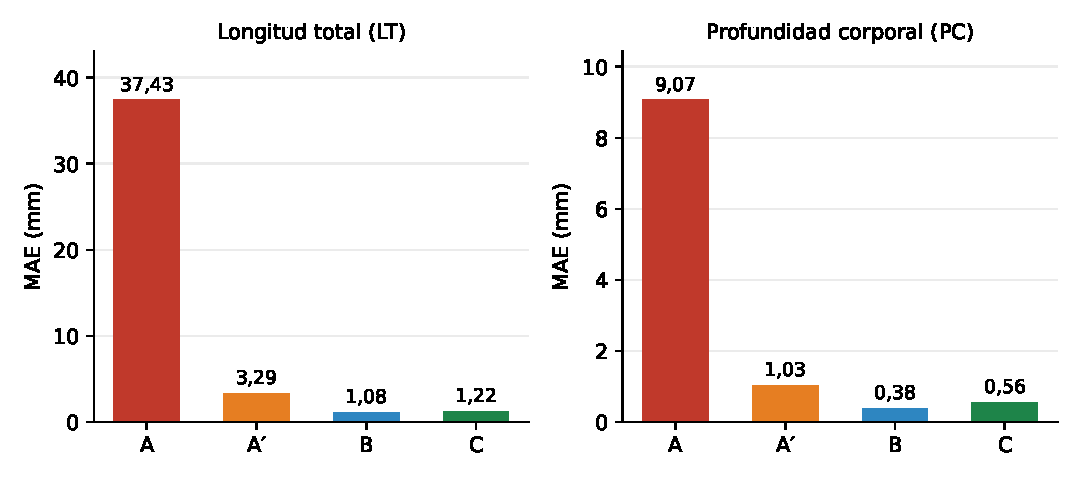
\includegraphics[width=\textwidth]{fig4_1_mae_por_metodo.pdf}
\caption[MAE por método para longitud total y profundidad corporal]{Error absoluto medio por método para longitud total (izquierda) y profundidad corporal (derecha), sobre las 24 combinaciones réplica--profundidad (datos de la Tabla~\ref{tab:agregados}). Fuente: elaboración propia.}
\label{fig:4-1}
\end{figure}

En LT, A subestimó en promedio 37,43~mm. La homografía de \Aprime{} redujo el MAE a 3,29~mm, y las dos rutas que usan la profundidad conocida con un modelo de cámara calibrado lo llevaron a 1,08~mm (B) y 1,22~mm (C). En PC se observó el mismo orden: A alcanzó un MAE de 9,07~mm, \Aprime{} de 1,03~mm, C de 0,56~mm y B de 0,38~mm. Calculado sobre las capturas individuales, el MAE de LT de B y C fue prácticamente igual (1,35 y 1,34~mm).

En la comparación pareada de LT, C tuvo menor error absoluto que A y que \Aprime{} en las 24 combinaciones, y B fue mejor que A en las 24 y que \Aprime{} en 23 (la excepción fue R2 a 5~cm). Con la réplica como unidad experimental, tanto B como C tuvieron menor error absoluto medio de LT que A y que \Aprime{} en las seis réplicas; la prueba de signos exacta de dos colas sobre las seis diferencias pareadas da $p = 2/2^{6} = 0{,}031$ en cada una de esas cuatro comparaciones. Entre B y C no hubo diferencia: C tuvo menor error de LT en 10 de las 24 combinaciones y en 3 de las 6 réplicas (R2, R5 y R6; $p = 1$). Los conteos sobre las 24 combinaciones se reportan como descriptivos porque las combinaciones de una misma réplica no son independientes. Para PC, C fue mejor que A en las 24 combinaciones y que \Aprime{} en 21 (5 de 6 réplicas, $p = 0{,}219$; la excepción fue R5, con un MAE de PC de 0,32~mm para \Aprime{} y 0,75~mm para C), y B fue mejor que C en 16 de las 24 combinaciones y en 5 de las 6 réplicas ($p = 0{,}219$), de nuevo con R5 como excepción.

\section{Comportamiento según la profundidad}
\label{sec:profundidad}

La dependencia con la distancia al vidrio se aprecia con mayor claridad en la longitud total. La Tabla~\ref{tab:posiciones-mae} presenta el MAE de LT para cada posición, calculado después de promediar las repeticiones técnicas, y la Figura~\ref{fig:4-2} muestra las cuatro curvas.

\begin{table}[htbp]
\centering\footnotesize
\caption{MAE de longitud total (mm) por posición de la réplica.}
\label{tab:posiciones-mae}
\begin{tabular}{@{}p{1.6cm}p{2.6cm}ccccc@{}}
\toprule
Distancia (cm) & Separación de la zona de B (cm) & A & \Aprime & B & C & B $-$ C \\
\midrule
5  & 0  & 13,77 & 3,44 & 1,18 & 1,09 & $+0{,}09$ \\
11 & 6  & 32,02 & 3,18 & 1,10 & 1,41 & $-0{,}31$ \\
17 & 12 & 46,29 & 3,44 & 1,01 & 1,29 & $-0{,}28$ \\
23 & 18 & 57,64 & 3,11 & 1,04 & 1,07 & $-0{,}04$ \\
\bottomrule
\end{tabular}
\end{table}

\begin{figure}[htbp]
\centering
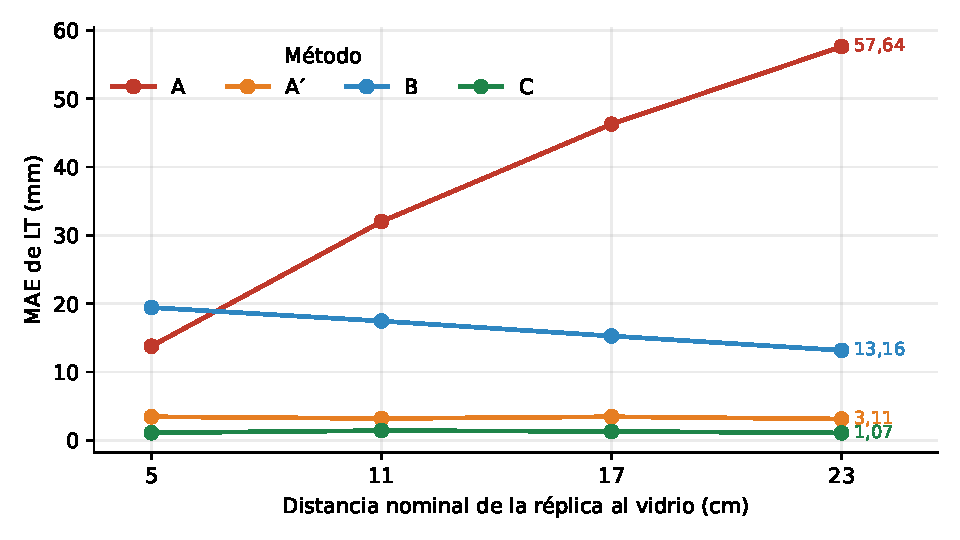
\includegraphics[width=0.9\textwidth]{fig4_2_mae_lt_profundidad.pdf}
\caption[MAE de longitud total por método y profundidad]{Error absoluto medio de longitud total por método y distancia de la réplica al vidrio (datos de la Tabla~\ref{tab:posiciones-mae}). El error de A crece con la profundidad; \Aprime, B y C se mantienen estables, y las curvas de B y C casi se superponen. Fuente: elaboración propia.}
\label{fig:4-2}
\end{figure}

El error de A aumentó de 13,77~mm a 5~cm hasta 57,64~mm a 23~cm, con una pendiente de 2,43~mm por centímetro de separación. Este comportamiento es compatible con una escala calculada en el plano del vidrio: al alejarse la réplica, la misma escala deja de representar adecuadamente su plano de medición. La predicción de primer orden de la ecuación~\eqref{eq:Dz} para una réplica de 140~mm da errores de $-19$, $-37$, $-50$ y $-60$~mm en las cuatro posiciones, frente a los $-14$, $-32$, $-46$ y $-58$~mm observados; la diferencia máxima, de 6~mm, es atribuible a que $d$ se midió desde el frente de la lente y a que las réplicas tienen longitudes distintas. Esta coincidencia es una verificación independiente del modelo óptico: el error de A es el que la geometría predice.

\Aprime{} se mantuvo cerca de 3,1--3,5~mm en todas las posiciones, lo que indica que el marcador coplanar redujo la variación asociada a la perspectiva. B permaneció entre 1,01 y 1,18~mm y C entre 1,07 y 1,41~mm, sin tendencia con la profundidad. La diferencia B $-$ C osciló entre $-0{,}31$ y $+0{,}09$~mm, con una pendiente de $-0{,}006$~mm por centímetro de separación: el error de B no aumentó al alejarse la réplica de la zona de calibración.

Para PC se observó un patrón equivalente para A: el MAE pasó de 3,02~mm a 5~cm a 14,24~mm a 23~cm. \Aprime{} varió entre 0,75 y 1,34~mm, B entre 0,25 y 0,48~mm y C entre 0,48 y 0,62~mm.

La Figura~\ref{fig:4-errores} muestra el error con signo de cada combinación réplica--profundidad, además de su media por posición. La dispersión de A crece con la profundidad junto con su sesgo; en LT, la de \Aprime{} fue de 4 a 5~mm alrededor de un sesgo positivo, y la de B y C fue similar entre sí, de 3,4 a 4,8~mm. Esa dispersión se repite entre posiciones para una misma réplica: R4 tuvo el mayor error absoluto de LT en \Aprime, B y C en las cuatro posiciones (en B y C, entre $+2{,}1$ y $+4{,}3$~mm), y su referencia de LT es una de las dos con mayor desviación entre lecturas (2,9~mm; Tabla~\ref{tab:replicas}). Esto apunta a la referencia de calibre o al marcado de esa réplica más que a la conversión.

\begin{figure}[htbp]
\centering
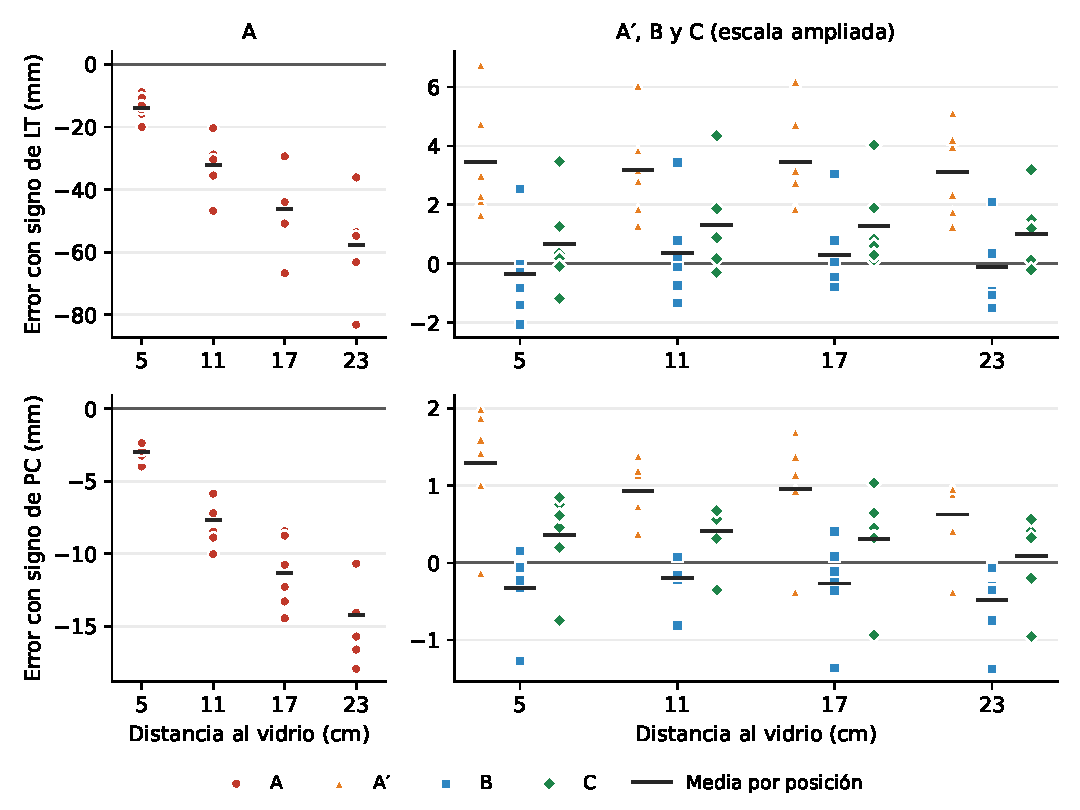
\includegraphics[width=\textwidth]{fig4_errores_combinaciones.pdf}
\caption[Error con signo por combinación réplica--profundidad]{Error con signo de LT (arriba) y PC (abajo) para cada una de las 24 combinaciones réplica--profundidad, después de promediar las repeticiones técnicas. A se presenta en un panel propio por su escala; \Aprime, B y C comparten un eje ampliado. Cada punto es una réplica y la línea horizontal, la media por posición. Fuente: elaboración propia.}
\label{fig:4-errores}
\end{figure}

\section{Repetibilidad del marcado manual}
\label{sec:repetibilidad}

\pendiente{Volver a marcar los cuatro puntos en doce imágenes (una por réplica a 5 y a 23~cm) sin consultar el marcado anterior, y completar la Tabla~\ref{tab:repetibilidad} con la diferencia media y máxima en píxeles por punto y su efecto en milímetros sobre LT y PC calculado con C. Cerrar con: «La repetibilidad del marcado introduce una variación de X~mm en LT, inferior/comparable al MAE de C y muy inferior a la diferencia entre métodos, por lo que las conclusiones de las Secciones~\ref{sec:agregados} y~\ref{sec:profundidad} no dependen del operador».}

\begin{table}[htbp]
\centering\footnotesize
\caption{Repetibilidad del marcado manual sobre doce imágenes remarcadas.}
\label{tab:repetibilidad}
\begin{tabular}{@{}p{3cm}p{2cm}p{2.2cm}p{3.2cm}p{1.6cm}@{}}
\toprule
Punto & Diferencia media (px) & Diferencia máxima (px) & Efecto medio en la medida (mm, con C) & Medida afectada \\
\midrule
$\mathbf{p}_1$ (hocico) & \pend{ } & \pend{ } & \pend{ } & LT \\
$\mathbf{p}_2$ (extremo caudal) & \pend{ } & \pend{ } & \pend{ } & LT \\
$\mathbf{p}_3$ (perfil dorsal) & \pend{ } & \pend{ } & \pend{ } & PC \\
$\mathbf{p}_4$ (perfil ventral) & \pend{ } & \pend{ } & \pend{ } & PC \\
\bottomrule
\end{tabular}
\end{table}

\section{Intervalo por profundidad desconocida}
\label{sec:intervalo}

La pregunta principal de este trabajo es qué intervalo de longitud puede garantizar C cuando la profundidad $z$ es desconocida y en qué condiciones ese intervalo es utilizable. Con el modelo de puerto plano, la longitud estimada para una misma imagen es una función $L(z)$ de la profundidad asumida; el intervalo $\IL$ de la ecuación~\eqref{eq:IL} recoge su variación sobre el rango admisible.

Para incidencia cercana a la normal, la magnificación de un punto situado a profundidad $z$ detrás del vidrio es, en primer orden, proporcional a $1/D(z)$, con $D(z) = d + t_g/\mu_g + z/\mu_w$ (ecuación~\ref{eq:Dz}), donde $d = 230$~mm, $t_g = 4$~mm, $\mu_g = 1{,}5$ y $\mu_w = 1{,}333$. Por tanto, $L(z)$ es proporcional a $D(z)$, creciente en $z$, y el intervalo puede escribirse como $[L(z_{\min}), L(z_{\max})]$. Esta misma relación reproduce el error observado de A dentro de 6~mm (Sección~\ref{sec:profundidad}), lo que respalda su uso para el intervalo.

Con ella, el ancho relativo de $\IL$ para una réplica situada a profundidad real $z_0$ es $(D(z_{\max}) - D(z_{\min}))/D(z_0)$. Para verificar esa predicción, C se ejecutó sobre las 72 capturas con el plano de medición en $z = 0, 10, 20, \ldots, 300$~mm. $L(z)$ resultó estrictamente creciente en las 72 capturas (Figura~\ref{fig:4-Lz}), lo que confirma que $\IL = [L(z_{\min}), L(z_{\max})]$. La Tabla~\ref{tab:intervalo} y la Figura~\ref{fig:4-3} presentan el ancho numérico, expresado como porcentaje de la LT de calibre, para las cuatro posiciones y tres escenarios de conocimiento de $z$: desconocida en toda la pecera (0--30~cm), conocida con $\pm 3$~cm y conocida con $\pm 1$~cm. La predicción de primer orden, que se indica entre paréntesis, difirió del cálculo numérico en 0,6~\% en promedio.

\begin{table}[htbp]
\centering\footnotesize
\caption{Ancho relativo del intervalo $\IL$ (\% de la LT de calibre) según la profundidad de la réplica y el conocimiento disponible sobre $z$: cálculo numérico con C sobre las 72 capturas y, entre paréntesis, predicción geométrica de primer orden. La última columna indica la cobertura empírica.}
\label{tab:intervalo}
\begin{tabular}{@{}lccccc@{}}
\toprule
Conocimiento de $z$ & 5~cm & 11~cm & 17~cm & 23~cm & Cobertura \\
\midrule
Desconocida (0--30~cm) & 81,8 (83,3) & 71,0 (71,4) & 62,4 (62,5) & 55,6 (55,5) & 1,00 \\
Conocida con $\pm 3$~cm & 16,4 (16,7) & 14,2 (14,3) & 12,5 (12,5) & 11,1 (11,1) & 1,00 \\
Conocida con $\pm 1$~cm & 5,5 (5,6) & 4,7 (4,8) & 4,2 (4,2) & 3,7 (3,7) & 0,81 \\
\midrule
MAPE de \Aprime{} ($z$ conocida) & \multicolumn{4}{c}{2,3} & \\
MAPE de B ($z$ conocida) & \multicolumn{4}{c}{0,7} & \\
MAPE de C ($z$ conocida) & \multicolumn{4}{c}{0,9} & \\
\bottomrule
\end{tabular}
\end{table}

\begin{figure}[htbp]
\centering
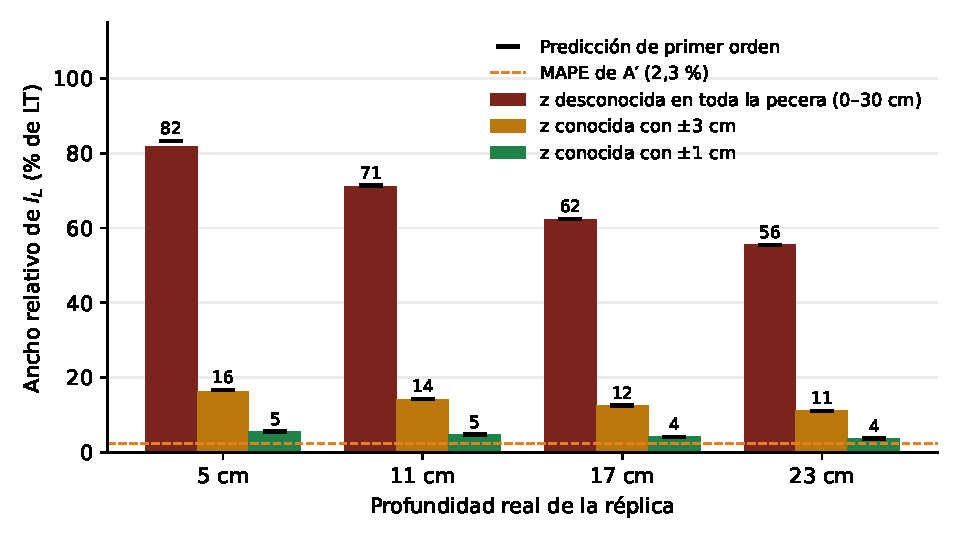
\includegraphics[width=0.9\textwidth]{fig4_3_ancho_intervalo.pdf}
\caption[Ancho relativo del intervalo por profundidad desconocida]{Ancho relativo del intervalo $\IL$ según la profundidad real de la réplica y el conocimiento disponible sobre $z$ (datos de la Tabla~\ref{tab:intervalo}). Las barras muestran el cálculo numérico y los marcadores negros la predicción de primer orden; la línea discontinua marca el MAPE de \Aprime{} con profundidad conocida. Fuente: elaboración propia.}
\label{fig:4-3}
\end{figure}

Con una sola cámara y sin información de profundidad, el intervalo abarca entre 56 y 82~\% de la longitud de la réplica: no es utilizable para morfometría. Si la profundidad se acota a $\pm 3$~cm (por ejemplo, con una guía o un tanque angosto), el ancho baja a 11--16~\%, todavía mayor que el error de \Aprime, B y C con $z$ conocida. Solo cuando la profundidad se conoce con $\pm 1$~cm el ancho (4--5~\%) se vuelve comparable con el error de \Aprime{} (2,3~\%) y queda dentro de un orden de magnitud del de B y C (0,7 y 0,9~\%). La cobertura empírica fue completa (72 de 72 capturas) en toda la pecera y con $\pm 3$~cm, pero bajó a 0,81 (58 de 72) con $\pm 1$~cm: con una ventana tan estrecha, el propio error de C con $z$ conocida basta para que la LT de calibre quede fuera del intervalo en algunas capturas. Este es el resultado que responde la pregunta principal: el modelo refractivo elimina el error de conversión, pero la profundidad sigue siendo la fuente dominante de incertidumbre y debe medirse o acotarse, no asumirse.

\begin{figure}[htbp]
\centering
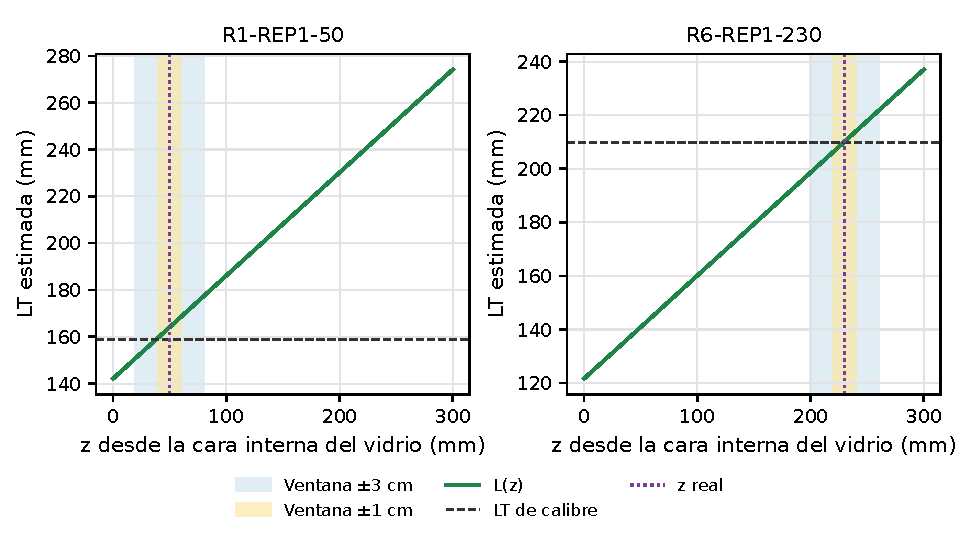
\includegraphics[width=0.9\textwidth]{fig4_L_z_ejemplos.pdf}
\caption[Longitud estimada por C en función de la profundidad supuesta]{Longitud total estimada por C en función de la profundidad supuesta $z$ para dos capturas (R1-REP1 a 5~cm y R6-REP1 a 23~cm). La línea discontinua horizontal indica la LT de calibre, la línea punteada vertical la profundidad nominal y las bandas las ventanas de $\pm 1$ y $\pm 3$~cm. Fuente: elaboración propia.}
\label{fig:4-Lz}
\end{figure}

\section{Contraste de hipótesis}
\label{sec:contraste}

La Tabla~\ref{tab:hipotesis} resume el contraste de las tres hipótesis con los criterios fijados en la Sección~\ref{sec:evaluacion}.

\begin{table}[htbp]
\centering\small
\caption{Contraste de hipótesis.}
\label{tab:hipotesis}
\begin{tabularx}{\textwidth}{@{}p{1.2cm} X X p{2.3cm}@{}}
\toprule
Hipótesis & Criterio & Valor observado & Veredicto \\
\midrule
H1 & Prueba de signos exacta por réplica, $p < 0{,}05$, para C frente a A, \Aprime{} y B en LT & Frente a A y \Aprime: C mejor en 6 de 6 réplicas ($p = 0{,}031$) y en 24 de 24 combinaciones. Frente a B: C mejor en 3 de 6 réplicas ($p = 1$) y en 10 de 24 combinaciones & Se sostiene frente a A y \Aprime; no frente a B \\
H2 & Pendiente positiva de $\mathrm{MAE}_B - \mathrm{MAE}_C$ frente a la separación & Pendiente $-0{,}006$~mm/cm ($+0{,}09$; $-0{,}31$; $-0{,}28$; $-0{,}04$~mm) & No se sostiene \\
H3 & Cobertura $\geq 0{,}95$ y ancho predicho dentro de la mitad del observado & Cobertura 1,00 (72 de 72) en toda la pecera; ancho numérico 56--82~\%, razón predicho/numérico 1,006 & Se sostiene \\
\bottomrule
\end{tabularx}
\end{table}

\paragraph{H1 se sostiene parcialmente.} C tuvo menor error absoluto de LT que A y \Aprime{} en las seis réplicas (prueba de signos exacta con la réplica como unidad, $p = 0{,}031$ en cada comparación) y en las 24 combinaciones réplica--profundidad (descriptivo), pero no que B: cada ruta fue mejor en tres réplicas ($p = 1$) y C lo fue en 10 de las 24 combinaciones. En PC, C fue mejor que A en 24 de 24 combinaciones y que \Aprime{} en 21 de 24, mientras que B fue mejor que C en 16 de 24. La parte de H1 que, en el protocolo, preveía equivalencia entre B y C dentro de la zona de calibración no se evaluó formalmente porque el margen $\delta$ no se fijó antes de observar los datos; a 5~cm el MAE de LT fue de 1,18~mm (B) y 1,09~mm (C), una diferencia de 0,09~mm, menor que la desviación de las referencias de calibre (Tabla~\ref{tab:replicas}) y compatible con que ambas rutas sean intercambiables en esa zona.

\paragraph{H2 no se sostiene.} La diferencia B $-$ C no aumentó con la separación ($+0{,}09$; $-0{,}31$; $-0{,}28$ y $-0{,}04$~mm; pendiente $-0{,}006$~mm/cm), y el MAE de B se mantuvo entre 1,01 y 1,18~mm en las cuatro posiciones. Hasta 18~cm de separación de la zona de calibración, la degradación con la distancia descrita por \textcite{Rofallski2022} no fue detectable con la resolución de este experimento; la interpretación se desarrolla en la Sección~\ref{sec:discusion}.

\paragraph{H3 se sostiene.} Con $z$ recorriendo toda la pecera, el intervalo $\IL$ contuvo la LT de calibre en las 72 capturas (cobertura 1,00), y el ancho predicho por la geometría del montaje difirió del calculado numéricamente en 0,6~\% en promedio, muy por debajo del margen de la mitad del ancho fijado en el criterio. La misma predicción reproduce el error de A dentro de 6~mm. Fuera del criterio de H3, la cobertura se mantuvo en 1,00 con $z$ acotada a $\pm 3$~cm y bajó a 0,81 con $\pm 1$~cm (Sección~\ref{sec:intervalo}).

\section{Discusión de los resultados}
\label{sec:discusion}

La comparación se realizó sobre los mismos puntos anatómicos y las mismas imágenes, por lo que la diferencia observada se relaciona principalmente con la transformación geométrica de cada ruta. La escala de A utiliza una referencia fija en el vidrio y no compensa la separación entre ese plano y el pez; el aumento de su error con la profundidad es el resultado más claro del conjunto y coincide con la predicción de primer orden del modelo óptico. \Aprime{} reduce ese efecto al trasladar la referencia al plano aproximado de la réplica, aunque sigue dependiendo de la calidad del marcado y de la coplanaridad conseguida. Conviene precisar la atribución causal: la diferencia entre A y \Aprime{} incluye tanto la coplanaridad del marcador como la rectificación por homografía, y la ventaja de B y C incluye la información de profundidad y, en C, el modelo completo de interfaces, no «la refracción» como causa única.

B presentó un sesgo prácticamente nulo en LT ($+0{,}05$~mm) y un MAE de 1,08~mm (0,73~\%) que no cambió con la separación de la zona de calibración. La calibración bajo agua absorbió la refracción en una focal efectiva (razón 1,36) y, con el plano de medición trasladado a lo largo del riel hasta la profundidad de cada captura, el modelo pinhole efectivo reprodujo la escala en todo el rango estudiado. Este resultado es coherente con la equivalencia de primer orden entre un puerto plano y una cámara pinhole con focal escalada (Sección~\ref{sec:calibraciones}): los efectos no centrales que \textcite{Rofallski2022} asocian a la distancia crecen con el ángulo de incidencia, y en este montaje, con las réplicas en la zona central del encuadre, quedaron por debajo de la resolución que imponen el marcado manual y la referencia de calibre.

B, al igual que C, necesita conocer la profundidad del plano de medición. En una ejecución preliminar, la lectura del riel se ingresó como distancia al vidrio, lo que alejó el plano 50~mm, y B sobreestimó la LT entre 13,3~\% (5~cm) y 9,1~\% (23~cm); el modelo de plano del riel predice esos valores dentro de 0,3 puntos porcentuales. La exactitud de B depende así de expresar la posición del pez en el mismo marco que la calibración, del mismo modo que la de C depende de la distancia $d$ (Tabla~\ref{tab:sensibilidad}).

B y C alcanzaron errores del mismo orden por vías distintas. B ajusta empíricamente una cámara efectiva con un patrón observado a través del agua y requiere una referencia del plano de medición en el marco de esa calibración; C modela las interfaces aire--vidrio--agua con parámetros físicos medidos ($d$, $t_g$ e índices) y una calibración en aire, que no depende del tanque. En LT ninguna fue mejor que la otra con la réplica como unidad, y la diferencia de MAE (0,14~mm) es menor que la desviación de las referencias de calibre; en PC, B tuvo menor MAE en 5 de 6 réplicas, sin significación ($p = 0{,}219$). La elección entre ambas es, por tanto, práctica: B exige calibrar dentro del tanque y referenciar el plano, y C exige medir $d$ con cuidado; C es, además, la ruta sobre la que se construyó el intervalo $\IL$. Tres evidencias respaldan la exactitud de C: la prueba de sanidad del módulo (con $\mu = 1$ y $t_g = 0$ reproduce la cámara pinhole), el error de 0,88~\% contra calibre en 72 imágenes y cuatro profundidades, y la coincidencia entre la predicción geométrica del error de A y lo observado. La exactitud de B y C se sostiene contra referencias físicas independientes del software (calibre) en 24 combinaciones; la comprobación complementaria con barra patrón, que permitiría separar un eventual error de implementación del error de marcado, queda como trabajo futuro.

Frente a los antecedentes, el error de B y C con profundidad conocida (MAE 1,08 y 1,22~mm; 0,7--0,9~\%) es menor que el informado por MorphoCal (MAE 7,5~mm, cámara sumergida y peces vivos; \citeauthor{Vijayalakshmi2026}, \citeyear{Vijayalakshmi2026}) y por \textcite{Seibold2026} (RMSE 6--9~mm, estéreo y peces vivos), pero las condiciones no son equivalentes: este trabajo usó réplicas rígidas, posturas controladas, puntos marcados a mano y una profundidad conocida por el soporte. La comparación válida no es entre cifras sino entre preguntas: los sistemas estéreo resuelven la profundidad con la segunda cámara; aquí se cuantificó qué se pierde al no tenerla.

La concordancia de C con el calibre se resume en la Figura~\ref{fig:4-BA}. Sobre las 24 combinaciones réplica--profundidad, C presentó en LT un sesgo de 1,07~mm con límites de acuerdo de $-1{,}73$ a 3,87~mm, y en PC un sesgo de 0,29~mm con límites de $-0{,}77$ a 1,35~mm. Sobre las 72 capturas individuales, que no son observaciones independientes, los límites fueron de $-2{,}42$ a 4,56~mm en LT y de $-1{,}01$ a 1,59~mm en PC. Para B, sobre las 24 combinaciones, el sesgo fue de 0,05~mm con límites de $-2{,}80$ a 2,90~mm en LT, y de $-0{,}32$~mm con límites de $-1{,}24$ a 0,61~mm en PC: B tuvo menor sesgo que C, pero límites de acuerdo de LT algo más amplios.

\begin{figure}[htbp]
\centering
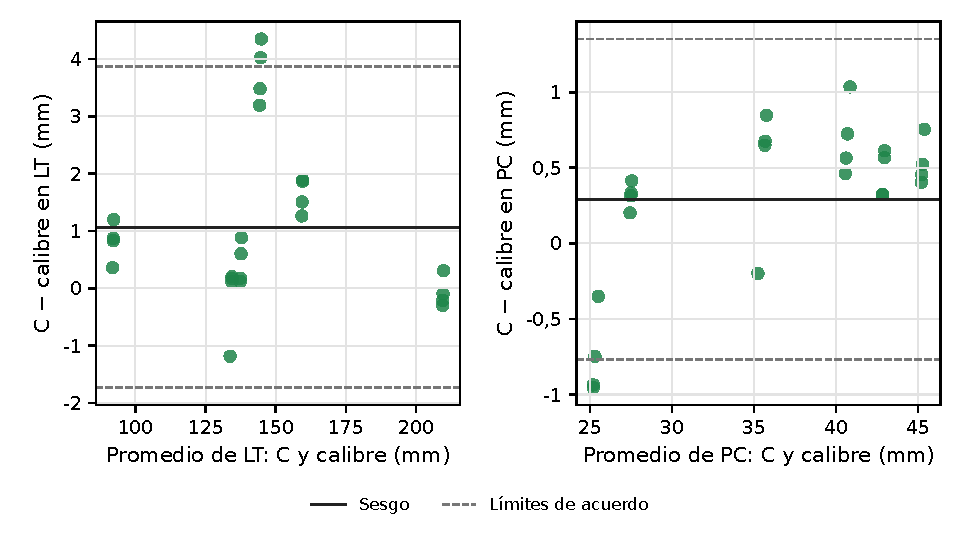
\includegraphics[width=0.95\textwidth]{fig4_bland_altman_c.pdf}
\caption[Bland--Altman de C frente al calibre]{Gráficos de Bland--Altman de C frente al calibre para LT (izquierda) y PC (derecha) sobre las 24 combinaciones réplica--profundidad. La línea continua indica el sesgo y las discontinuas los límites de acuerdo del 95~\%. Fuente: elaboración propia.}
\label{fig:4-BA}
\end{figure}

La Figura~\ref{fig:4-captura} muestra una de las capturas procesadas, con los cuatro puntos marcados y las estimaciones de cada ruta.

\begin{figure}[htbp]
\centering
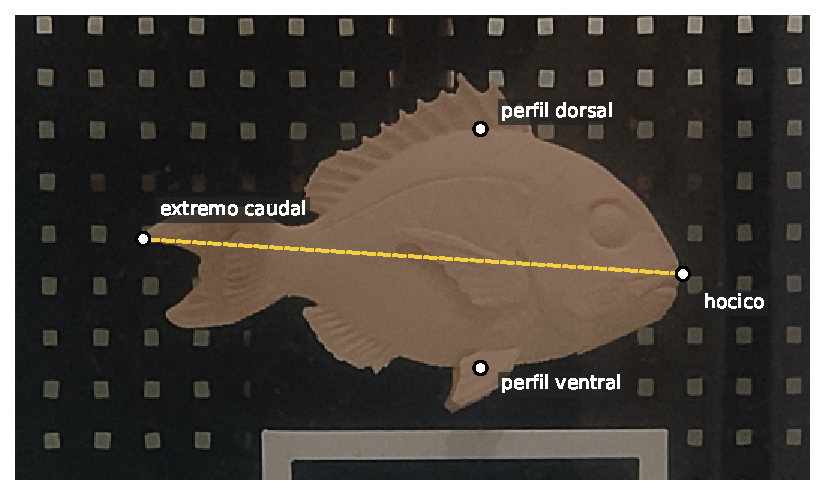
\includegraphics[width=0.9\textwidth]{fig4_captura_R3_230.pdf}
\caption[Captura real con los cuatro puntos anatómicos marcados]{Captura \texttt{R3-REP1-230.jpg} (réplica R3 a 23~cm del vidrio) con los cuatro puntos anatómicos marcados y el eje longitudinal. Referencia de calibre: LT 91,7~mm y PC 40,3~mm. Estimaciones de LT y PC: A, 55,4 y 24,5~mm; \Aprime, 93,7 y 41,6~mm; B, 91,7 y 40,1~mm; C, 92,6 y 40,7~mm. Fuente: elaboración propia.}
\label{fig:4-captura}
\end{figure}

\section{Alcance de los resultados}

Los resultados son válidos para las seis réplicas rígidas, la cámara Realme C71, la pecera de vidrio, las cuatro posiciones y las condiciones de iluminación utilizadas. No se generalizan directamente a peces vivos, movimiento, turbidez, oclusiones ni posiciones laterales que no fueron incluidas en la captura. Del mismo modo, las tres capturas técnicas no deben interpretarse como tres unidades experimentales independientes, y las 24 combinaciones réplica--profundidad no son 24 unidades: la unidad experimental es la réplica ($n = 6$).

En conjunto, los datos respaldan una ventaja de B y C, con la profundidad conocida, y en segundo lugar de \Aprime, frente a A para las medidas analizadas; entre B y C no se encontró diferencia en LT. Estas conclusiones se apoyan en la réplica como unidad y en referencias físicas de calibre. La conclusión se limita al flujo de procesamiento, al montaje y a las referencias físicas registradas.
